In the tau reconstruction, $\tauhad$ candidates are seeded from jets. Therefore, QCD events represent the main source of background (BG). Nonetheless, we do not have MC simulations for this processes. For this reason, we use a \textit{data driven method} to estimate multi-jet (MJ). In this section we will discuss how we derived our Multi-Jet Background (MJBG) estimation.

\subsection{Multi-Jet Background}
To obtain the MJBG, a variable that in principle is supposed to be uncorrelated with the shape of the MJBG is chosen. For our study, this variable is the relative sign between the charges of the $\tauhad$ and the lepton. This defines two regions: the same sign (SS) region where $q(\tauhad)=q(l)$ and the opposite sign region where $q(\tauhad)=-q(l)$. Our estimate for the MJBG in the SS region is obtained by subtracting signal and electroweak backgrounds (EWBG) contributions:
\begin{equation}
\text{MJBG}_{\text{SS}}=\text{Data}_{\text{SS}}-\text{Signal}_{\text{SS}}-\text{EWBG}_{\text{SS}},
\label{eq19}
\end{equation}
To study the residual charge correlation, we define a control region (CR) where the MJ background is enhanced. The estimate for the MJBG in these regions is given by eq. \ref{eq19} as well. The region described in Sec.\ref{sec3.3}, which contains all our final selected events is called the signal region (SR). In contrast to the SR, the CR is defined by events that fail the lepton isolation criteria and that fail the Tight-ID working point criterion for the $\tauhad$ candidate. In this region, tau candidates are required to have a looser tau-$pt$ of 25 GeV or more. This last choice was made to increase the number of candidates in the CR. The other kinematic features of the SR are maintained. A diagram showing the four regions just defined is shown in Fig.\ref{Fig7}. Now, if we assume that charge correlation is the same in the SR and CR, we have:
 \begin{equation}
 \frac{\text{MJBG}_{\text{SR OS}}}{\text{MJBG}_{\text{SR SS}}}=\frac{\text{MJBG}_{\text{CR OS}}}{\text{MJBG}_{\text{CR SS}}},
 \end{equation}
then,
 \begin{equation}
\text{MJBG}_{\text{SR OS}}=\text{MJBG}_{\text{SR SS}}\times \text{RQCD}\,
\label{eq36}
\end{equation}
where $\text{RQCD}\equiv\frac{\text{MJBG}_{\text{CR OS}}}{\text{MJBG}_{\text{CR SS}}}$. So, \eqref{eq36} gives the estimation of MJBG on the SROS.
\begin{figure}[htbp]
	\centering
	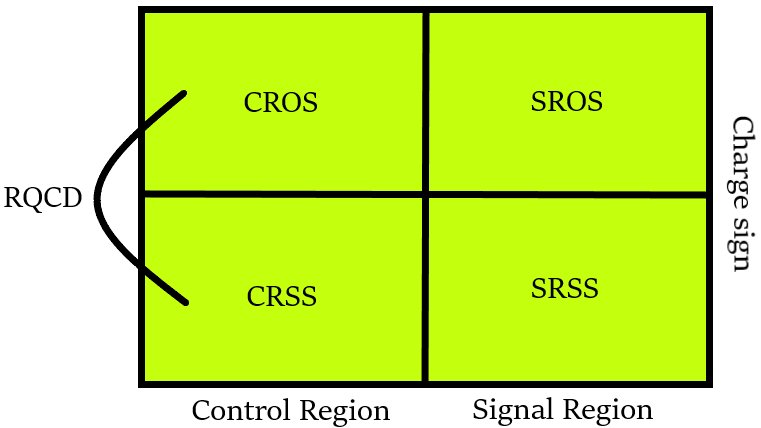
\includegraphics[width=0.5\textwidth]{figures/Fig7.png}
	\caption{Regions defined to estimate MJ background contribution in the SROS region. This data-driven method is also known as the ABCD method.}
	\label{Fig7}
\end{figure}
Table \ref{tab:MJ} summarises inputs into the calculation of the MJ background in the three candidate event samples. 

\begin{table}[]
	\resizebox{\textwidth}{!}{%
		\begin{tabular}{ccccc}
			\rowcolor[HTML]{C0C0C0} 
			\textbf{Sample} & \multicolumn{2}{c}{\cellcolor[HTML]{C0C0C0}\textbf{$\mu \tauhad$}} & \multicolumn{2}{c}{\cellcolor[HTML]{C0C0C0}\textbf{$e \tauhad$}} \\
			& 1-prong                                  & 3-prong                                 & 1-prong                                 & 3-prong                                \\ \hline
			CR OS Data      & 476.0 $\pm$ 22                                 & 270.0 $\pm$ 16                               & 62.0  $\pm$ 8                               & 39.0 $\pm$ 6                               \\
			MC              & 28.608 $\pm$                                & 10.531 $\pm$                               & 21.058 $\pm$                               &              4.794 $\pm$                  \\
			CR SS Data      & 366.0 $\pm$ 19                                 & 151.0 $\pm$ 12                                 & 56.0 $\pm$ 7                                & 28.0 $\pm$ 5                                \\
			MC              & 3.46 $\pm$                                 & 0.381 $\pm$                                  & 1.152 $\pm$                                &                    0.843 $\pm$             \\ \hline
			RQCD            & 1.234 $\pm$ 0.081                                  & 1.723 $\pm$ 0.178                                 & 0.746 $\pm$ 0.208                                  & 1.260 $\pm$ 0.342                                \\ \hline
			SR SS Data      & 95.0 $\pm$ 10                                  & 13.0 $\pm$ 4                                  & 113.0 $\pm$ 11                                 & 18.0 $\pm$ 4                                 \\
			MC              & 57.257 $\pm$                                 & 6.761 $\pm$                                   & 63.585 $\pm$                                & 19.240 $\pm$                                \\ \hline
			MJ Background   & 46.577 $\pm$  13.825	                               & 10.748 $\pm$ 13.870                                & 36.887 $\pm$  15.695                              & 0.0 $\pm$ 15.695                                 
		\end{tabular}%
	\caption{Inputs for the calculation of the central value of the MJBG yield in the two final states, $Z\to\mu\tauhad$ and $Z\to e\tauhad$.
		The numbers of data events in the CR OS and CR SS samples are given, together with the total numbers of events in these
		categories expected from simulation.
		The excess of data with respect to simulation is assumed to arise from MJBG and it is used to calculate the value of RQCD.
	}

	\label{tab:MJ}
}





\end{table}

Fig. \ref{Fig12} shows the jetRNN score distributions for the events in the CRs. It can be seen that the samples are dominated by non-simulated background.

\begin{figure}[htbp]
	\centering
	\subfloat[]{\label{Fig12a}{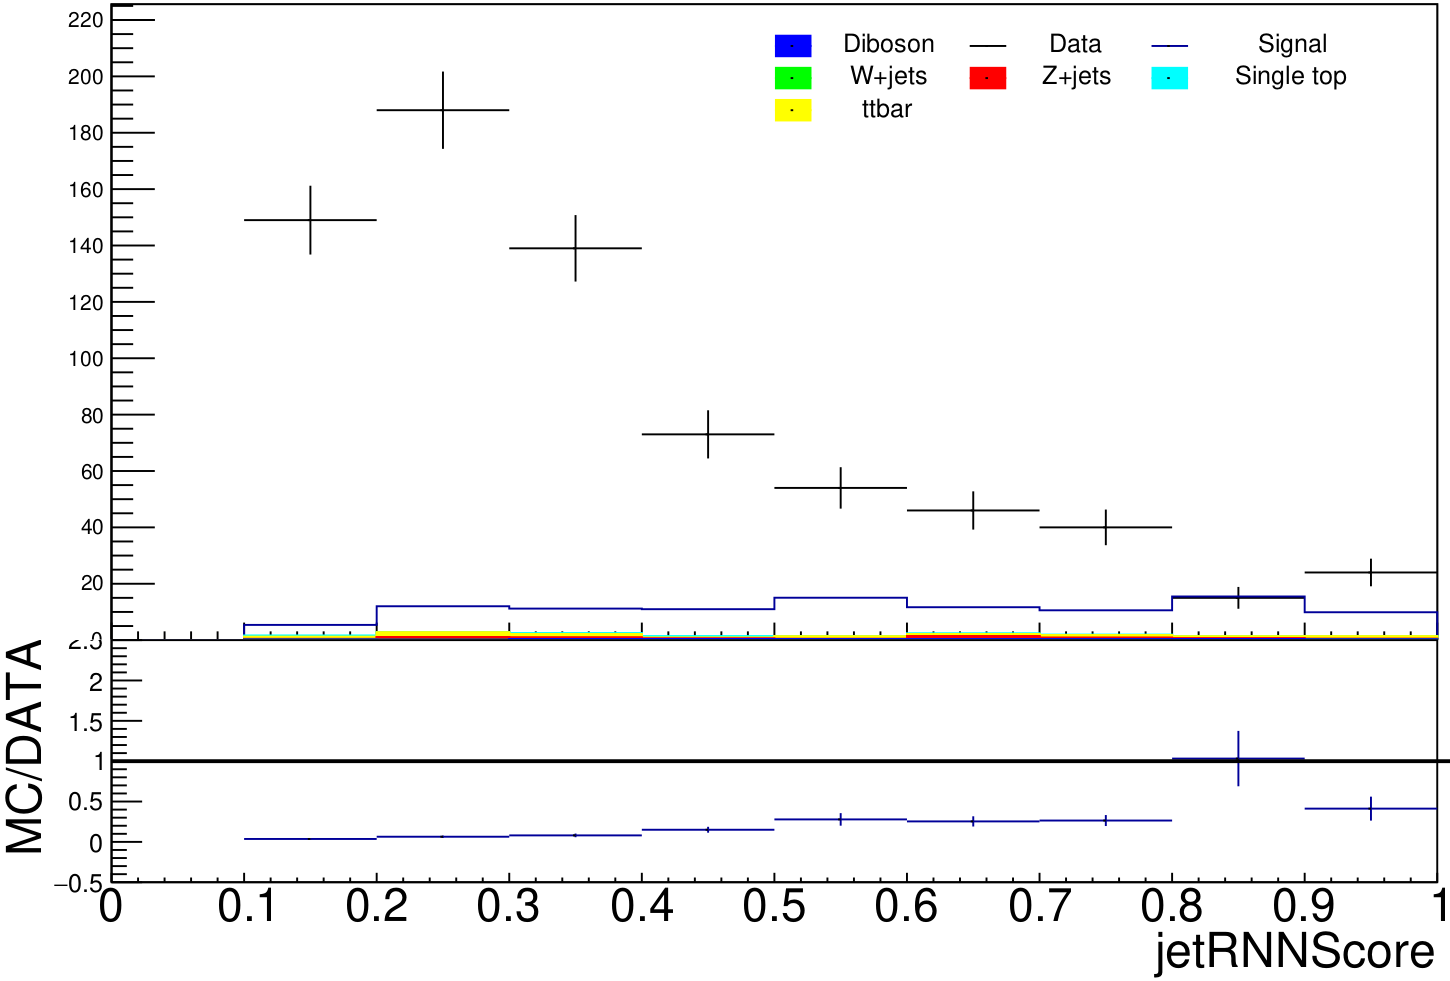
\includegraphics[width=0.50\textwidth]{figures/Fig12a.png}}}
	\subfloat[]{\label{Fig12b}{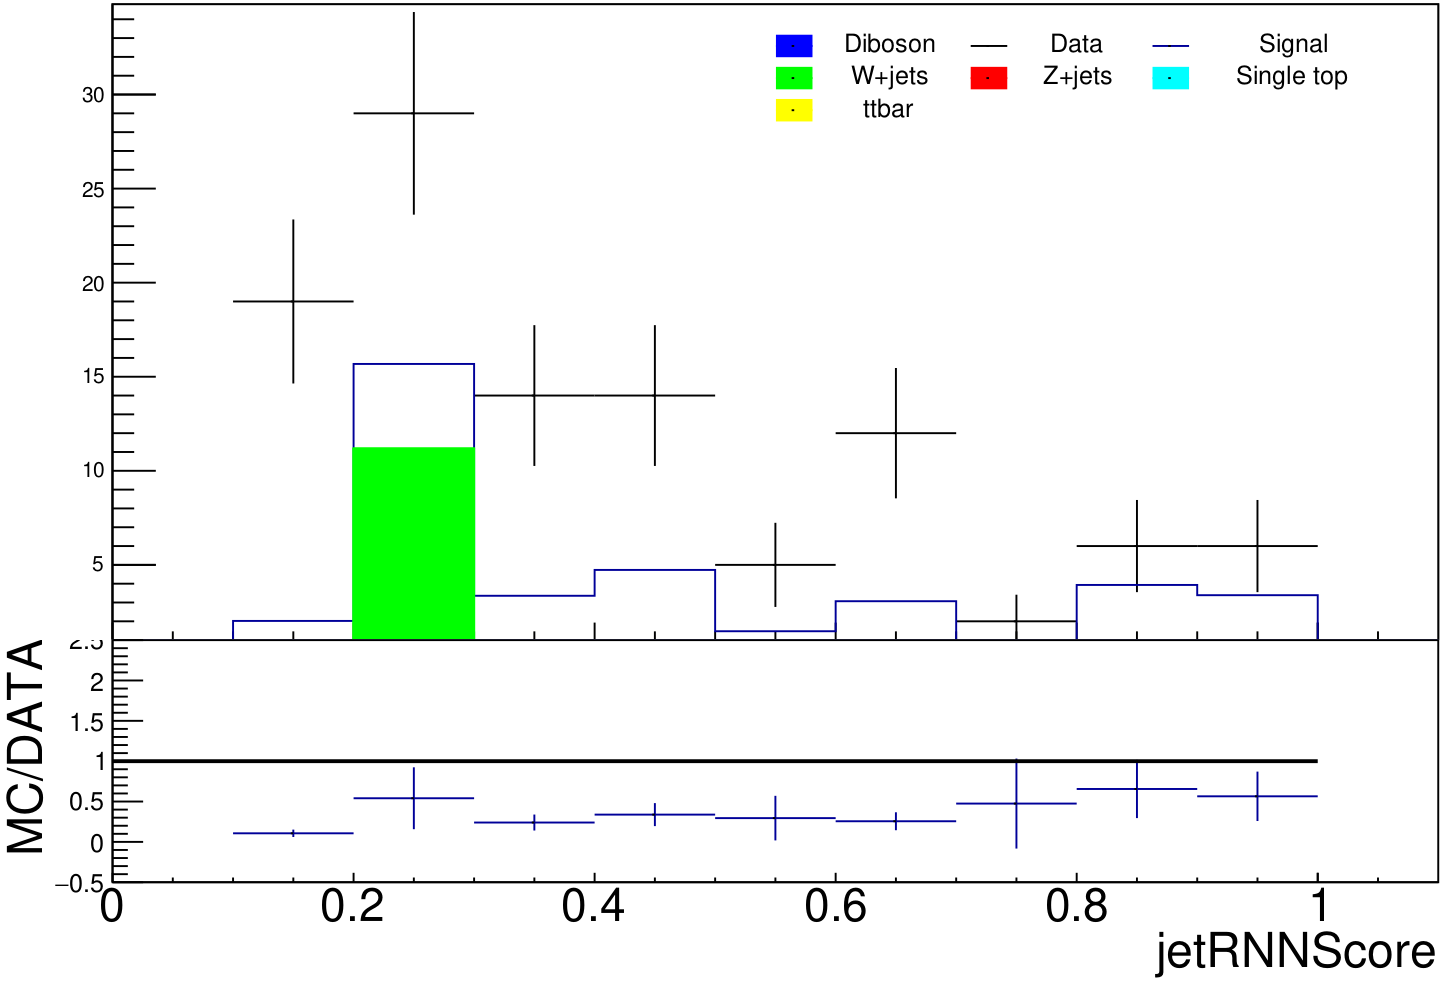
\includegraphics[width=0.50\textwidth]{figures/Fig12b.png}}}\hfill
	\subfloat[]{\label{Fig12c}{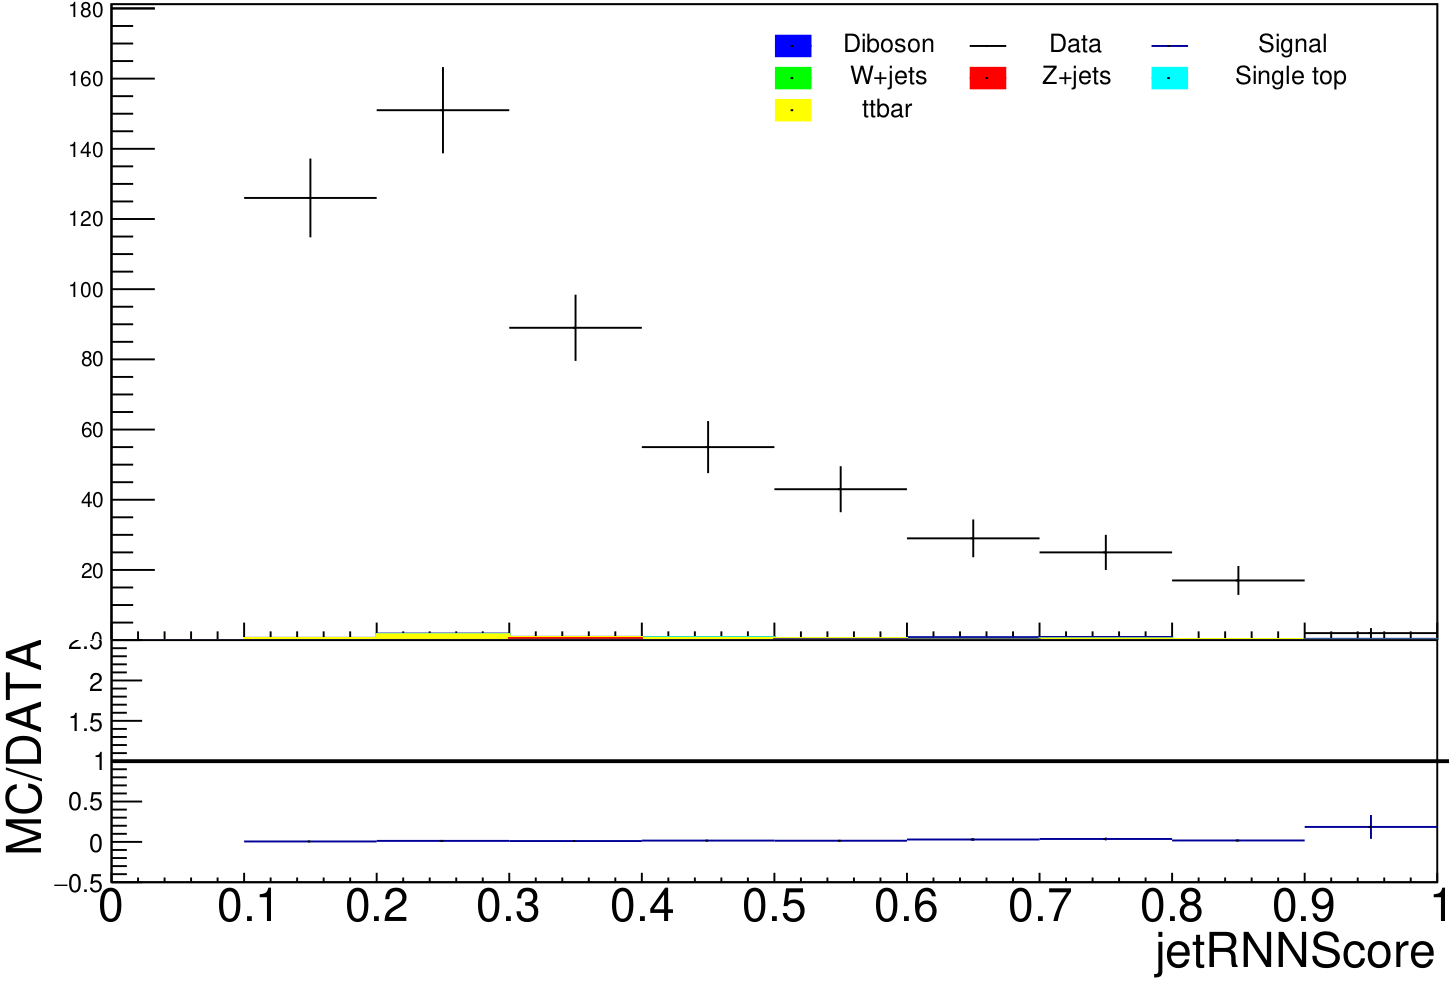
\includegraphics[width=0.50\textwidth]{figures/Fig12c.png}}}
	\subfloat[]{\label{Fig12d}{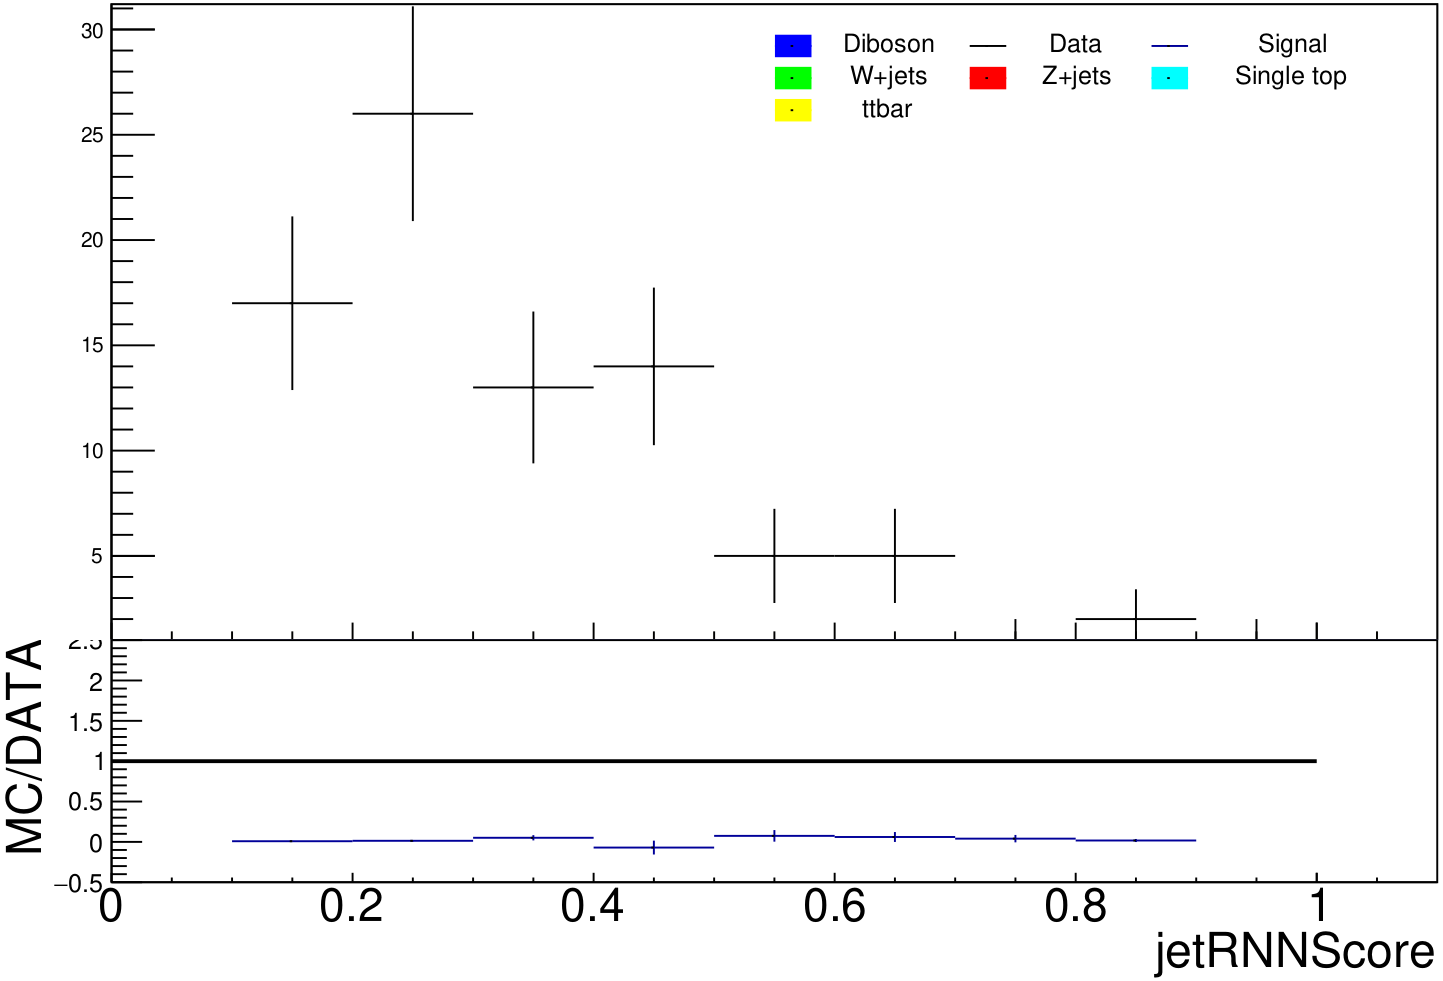
\includegraphics[width=0.50\textwidth]{figures/Fig12d.png}}}
	\caption{Left column (a,c) represents $Z\to\tauhad\mu$ and $Z\to\tauhad e$ is in the right column (b,d). The two figures on top show the CROS and the bottom ones represent the CRSS. All of the plots show the jetRNNScore for 1 prongs. In this case the events used to calculate RQCD are the ones with jetRNNScore$<0.4$.  }
	\label{Fig12}
\end{figure}

\subsection{Electroweak Background}
The electroweak background (EWBG) sources considered are $t\bar{t}$, $\Zjets$, Diboson and single top processes. For all of them, simulated samples are available and they are listed in Table \ref{Table3}. At an early stage of our analysis the $\Wjets$  simulation was checked for correctly accounting for the expected EWBG. This study is described in Appendix \ref{wjetsstudy}. Nonetheless, the final $\Wjets$ contribution to our background yield is so small that an updated study will not improve the quality and precision of our results.  